% Build:  pdflatex nominal_N2_report.tex   (twice, from this directory)
\documentclass[11pt,a4paper]{article}

\usepackage[margin=2.3cm]{geometry}
\usepackage[T1]{fontenc}
\usepackage{lmodern}
\usepackage{microtype}
\usepackage{amsmath,amssymb}
\usepackage{graphicx}
\usepackage{booktabs}
\usepackage{subcaption}
\usepackage[font=small,labelfont=bf]{caption}
\usepackage{titlesec}
\usepackage[colorlinks=true,linkcolor=black,citecolor=black]{hyperref}

\graphicspath{{../figs/}}

\titleformat{\section}{\normalfont\large\bfseries}{\thesection}{0.7em}{}
\titlespacing*{\section}{0pt}{1.4ex plus .3ex}{0.8ex}

\newcommand{\code}[1]{\texttt{\small #1}}
\newcommand{\Teff}{T_{\mathrm{eff}}}
\newcommand{\vperp}{v_\perp}
\newcommand{\vpar}{v_\parallel}
\setlength{\parskip}{0pt}
\setlength{\textfloatsep}{8pt plus 2pt minus 2pt}
\setlength{\intextsep}{8pt plus 2pt minus 2pt}
\setlength{\floatsep}{8pt plus 2pt minus 2pt}
\setlength{\abovecaptionskip}{4pt}
\setlength{\belowcaptionskip}{0pt}

\title{\vspace{-1.2cm}\textbf{\large Second-harmonic minority ICRF heating in ITER-EDA}\\[1mm]
\normalsize The nominal $N{=}2$ reference case}
\author{\normalsize F.~Louche}
\date{\normalsize 19 August 2026}

\begin{document}
\maketitle
\vspace{-0.9cm}

\begin{abstract}
\noindent\small
The reference second-harmonic ITER-EDA case is a mass-3 minority at $50\%$
concentration in deuterium, heated at $60.9\,$MHz with the rigorous non-linear
self-collision operator. It reaches a steady state in $12.5\,$s of physical
time, at an effective temperature of $32.59\,$keV against a $12\,$keV bulk, with
$73.9\%$ of the tail energy perpendicular. The absorbed power density is
$1.82\,$MW/m$^3$, shed to the background ions and to the electrons in the ratio
$59{:}41$. The RF fills the tail on $0.22\,$s, faster than either collisional
channel drains it, which is what sustains the supra-thermal population.
\end{abstract}

\vspace{-0.3cm}
\section{Configuration}

A tritium-like minority (mass 3, $Z{=}1$) in a deuterium majority, both at
$50\%$ of $n_e=1.5\times10^{20}\,$m$^{-3}$, with $T_e=T_i=12\,$keV and
$B_0=6\,$T. The wave is applied at the second cyclotron harmonic
(Table~\ref{tab:setup}). Self-collisions use the non-linear operator built from
the Rosenbluth potentials of the evolving distribution (\code{isc = -1}); the
time-differencing weight is $\theta=0.75$ (\code{icn = 1}).

\begin{table}[h]
\centering\small
\caption{Case parameters. The run terminated on the \code{conv\_diag} criteria
at $t=12.5\,$s after $276\,$s of wall time.}
\label{tab:setup}
\begin{tabular}{@{}llll@{}}
\toprule
harmonic & $N=2$ & grid & $150\times150$, quadratic in $\vperp$ \\
frequency & $60.9\,$MHz & $\vperp^{\max}$ & $3.0\times10^{7}\,$m/s \\
$k_\perp$, $k_\parallel$ & $40$, $2\,$m$^{-1}$ & $\vpar$ range & $[-8,8]\times10^{6}\,$m/s \\
$E_+$ & $(1300,100)\,$V/m & minority & mass 3, $Z=1$, $50\%$ \\
$E_-$ & $(3900,1)\,$V/m & majority & deuterium, $50\%$ \\
\bottomrule
\end{tabular}
\end{table}

\vspace{-0.2cm}
\section{The steady distribution}

Figure~\ref{fig:fout} shows the converged distribution. The RF builds a
pronounced perpendicular tail: $f$ falls by some fourteen decades between the
bulk and $\vperp\simeq25\,$Mm/s, and the contours are strongly elongated in
$\vperp$, the signature of a $J_1$-weighted quasi-linear operator depositing its
energy in a narrow band at high perpendicular velocity. The parallel direction
is barely heated.

\begin{figure}[h]
\centering
\begin{subfigure}{0.49\textwidth}\centering
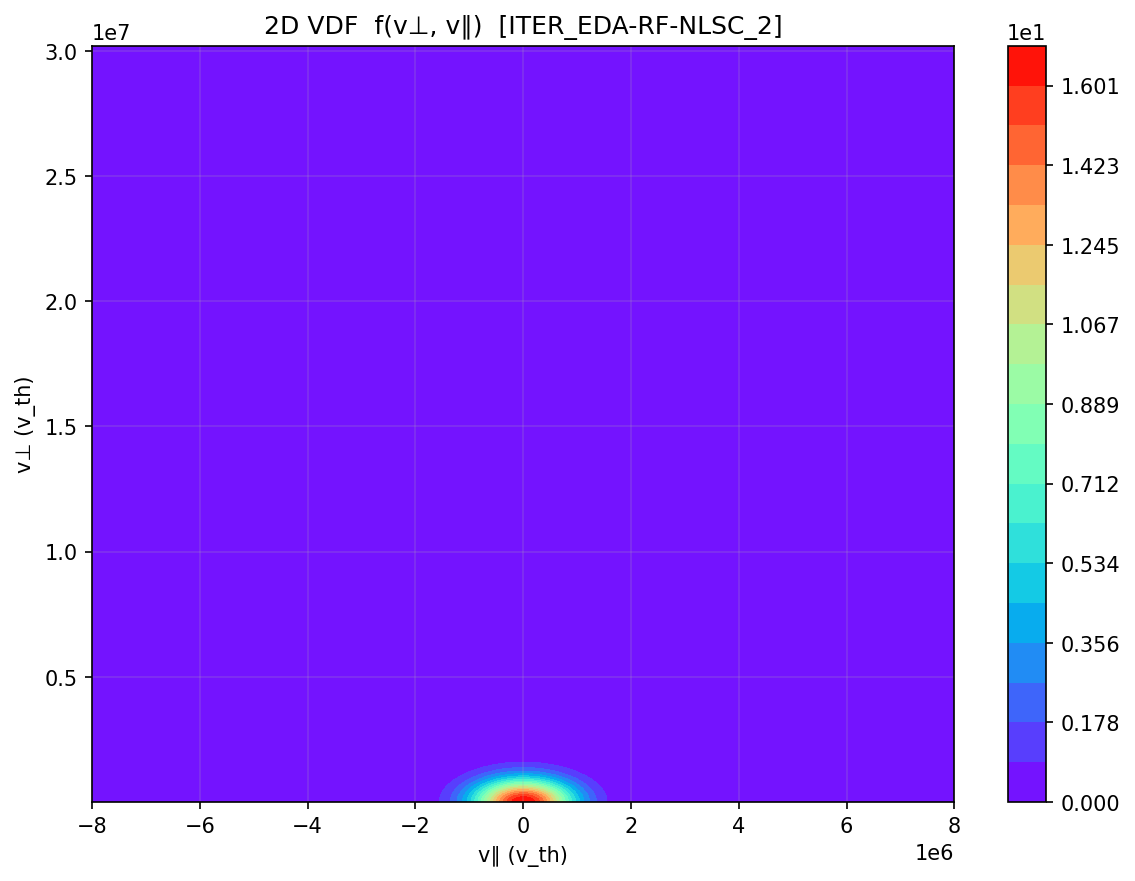
\includegraphics[width=\linewidth]{fout-ITER_EDA-RF-NLSC_2.png}
\caption{$f(\vperp,\vpar)$}
\end{subfigure}\hfill
\begin{subfigure}{0.49\textwidth}\centering
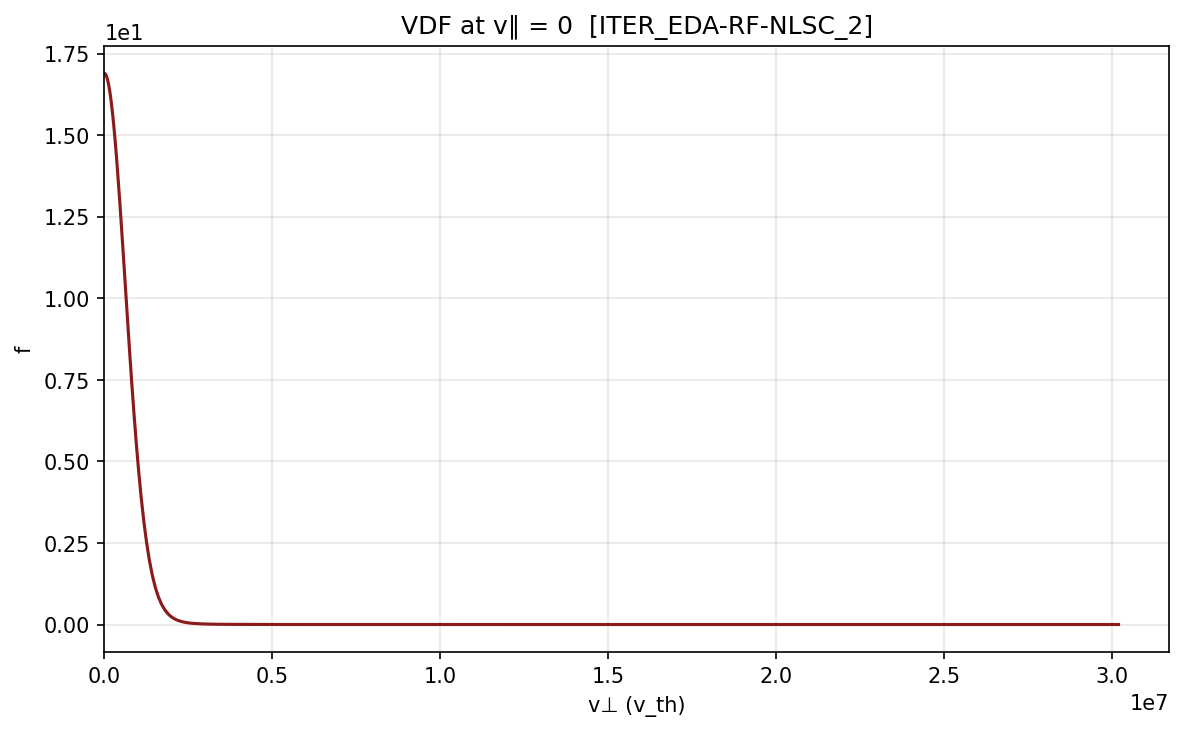
\includegraphics[width=\linewidth]{fout_at_vpar0-ITER_EDA-RF-NLSC_2.png}
\caption{cut at $\vpar=0$}
\end{subfigure}
\caption{Converged minority distribution. The perpendicular tail extends to
$\sim25\,$Mm/s, some forty times the $0.62\,$Mm/s thermal velocity of the
initial Stix Maxwellian.}
\label{fig:fout}
\end{figure}

\vspace{-0.2cm}
\section{Approach to steady state}

The effective temperature rises from the $12.2\,$keV initial condition to
$32.59\,$keV, and the anisotropy from $50.7\%$ --- essentially isotropic --- to
$73.9\%$ (Fig.~\ref{fig:evol}). Both saturate by $t\simeq8\,$s. The two
quantities are not equivalent: $\Teff$ nearly triples while the
density-characteristic temperature $T_n$ moves only from $12.1$ to $13.7\,$keV,
because $T_n$ is set by the bulk of the population and $\Teff$ by its second
moment, which the tail dominates.

\begin{figure}[h]
\centering
\begin{subfigure}{0.49\textwidth}\centering
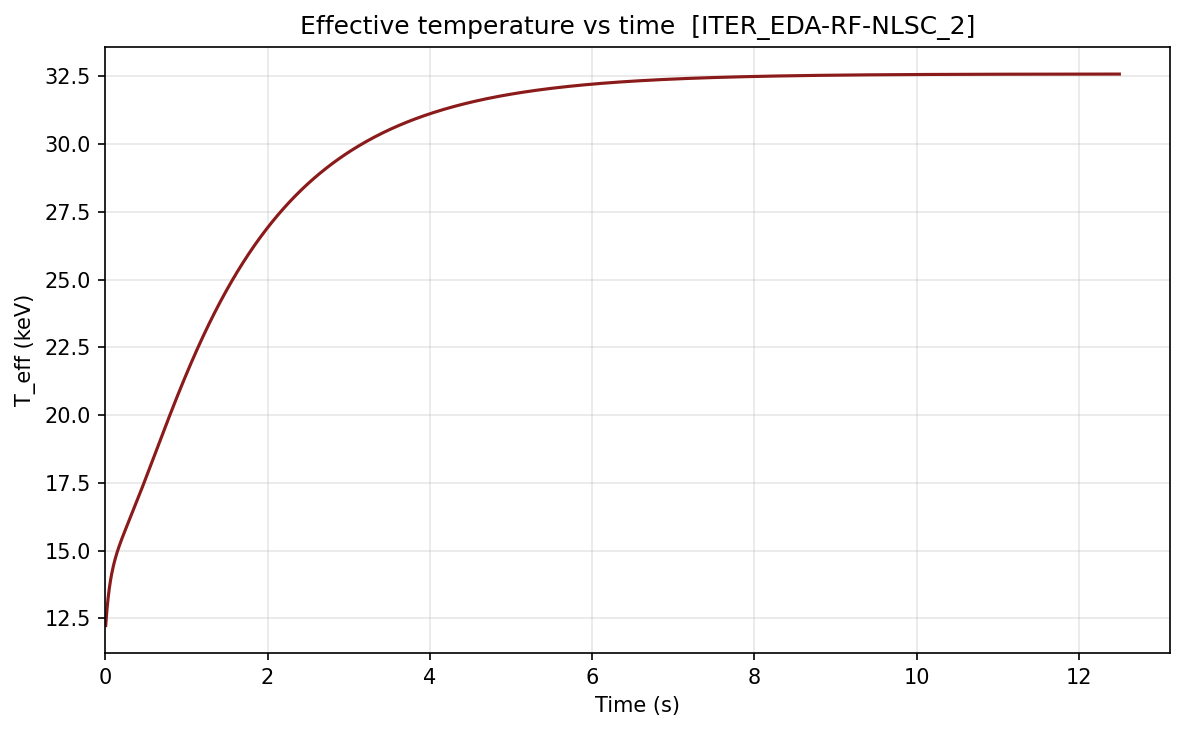
\includegraphics[width=\linewidth]{Teff_vs_time-ITER_EDA-RF-NLSC_2.png}
\caption{effective temperature}
\end{subfigure}\hfill
\begin{subfigure}{0.49\textwidth}\centering
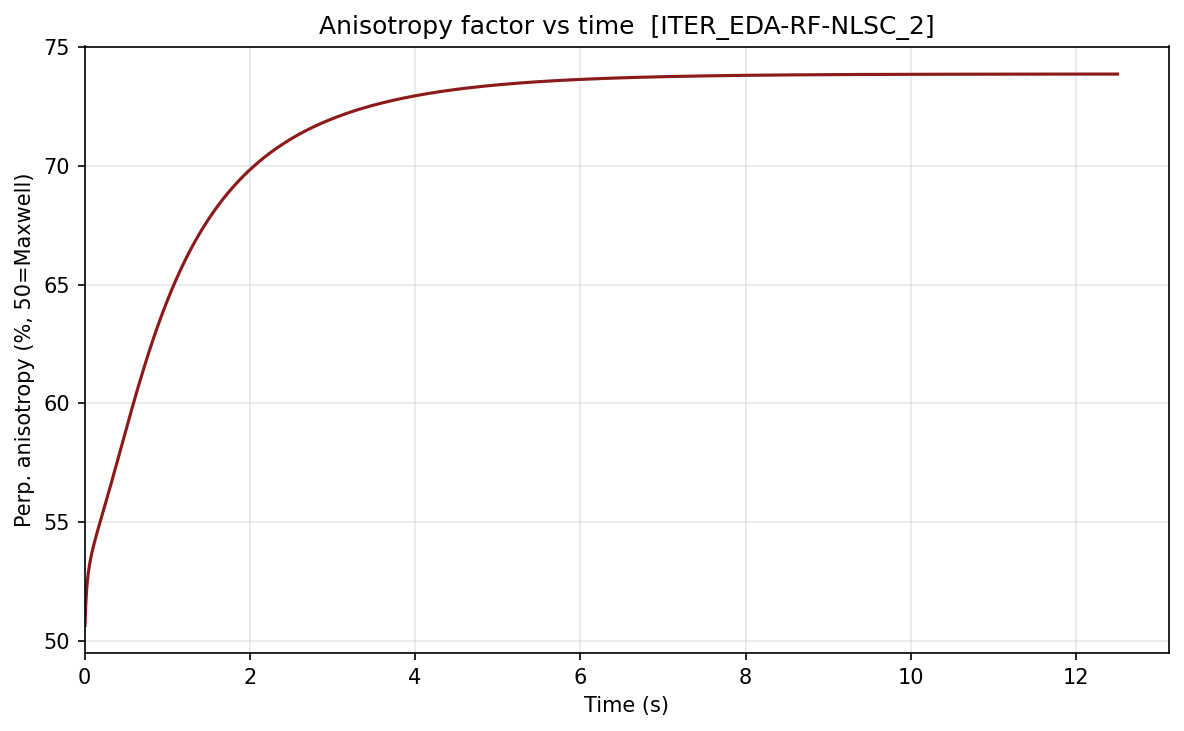
\includegraphics[width=\linewidth]{anisotropy_vs_time-ITER_EDA-RF-NLSC_2.png}
\caption{perpendicular anisotropy}
\end{subfigure}
\caption{Approach to steady state; $50\%$ anisotropy would be isotropic.}
\label{fig:evol}
\end{figure}


\vspace{-0.2cm}
\section{Power balance and timescales}

At steady state the RF supplies $1.8166\,$MW/m$^3$ and the collisions remove
$1.8166\,$MW/m$^3$, closing to $0.003\%$ (Fig.~\ref{fig:power}, left). The split
is $1.075\,$MW/m$^3$ to the background ions and $0.742$ to the electrons, or
$59{:}41$. That ordering is expected here: the critical energy for this minority
is $E_c\simeq106\,$keV, and at $\Teff=32.6\,$keV the tail sits well below it, so
ion drag still leads. Self-collisions carry no net energy --- they remove
$0.176\,$MW/m$^3$ from the perpendicular direction and return exactly the same
to the parallel, closing to $0.014\%$ --- but they are what couples the
RF-driven perpendicular tail to the parallel direction and hence to the bulk.

\begin{figure}[h]
\centering
\begin{subfigure}{0.49\textwidth}\centering
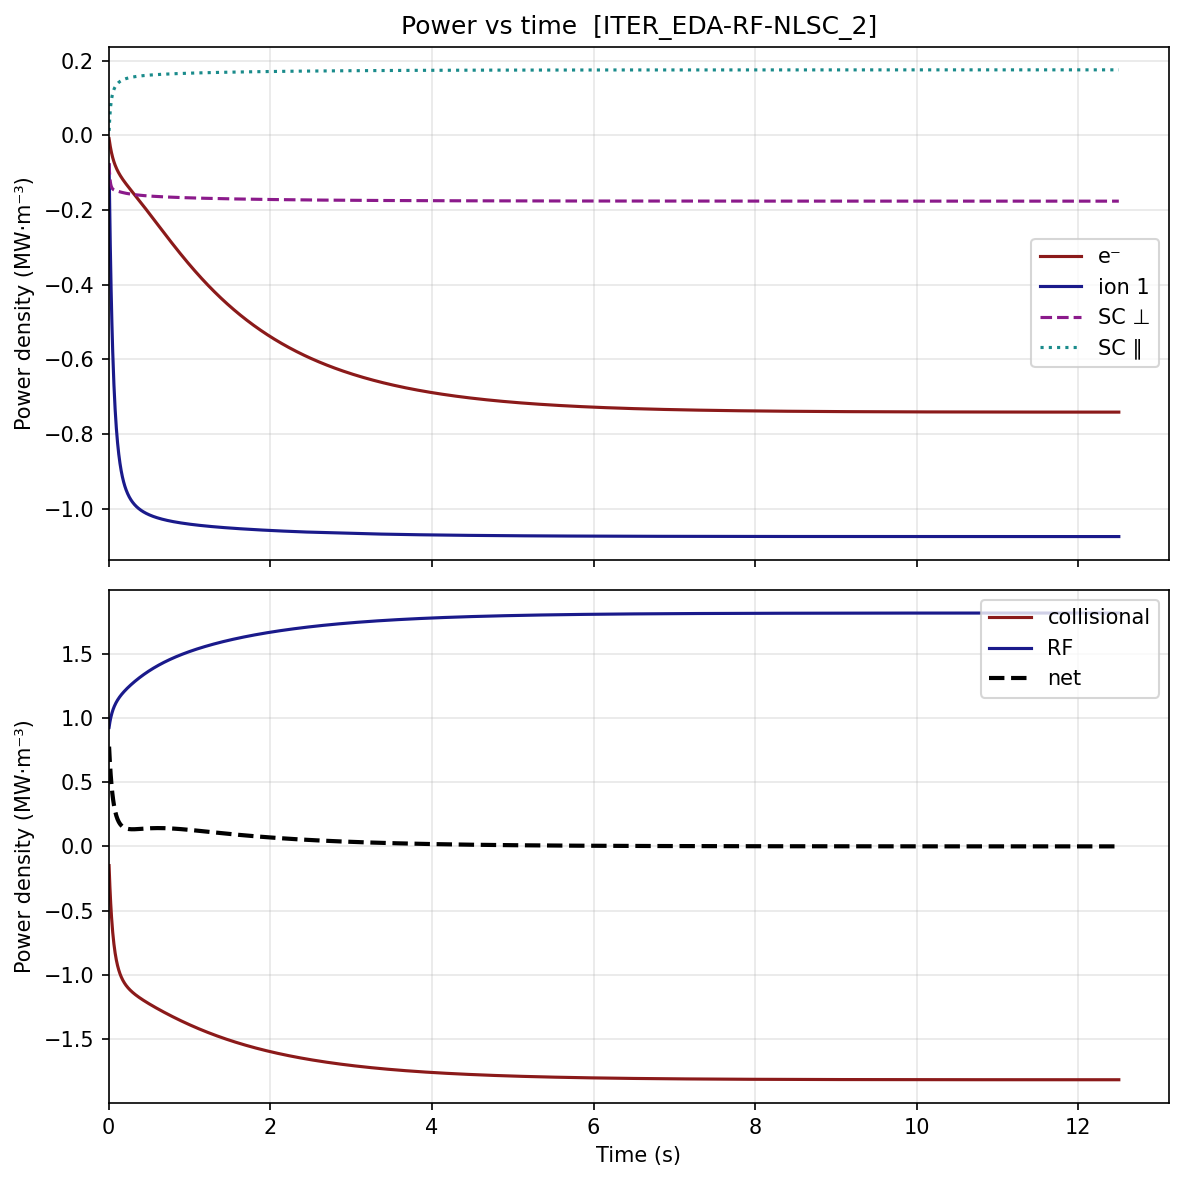
\includegraphics[width=\linewidth]{power_vs_time-ITER_EDA-RF-NLSC_2.png}
\caption{power balance}
\end{subfigure}\hfill
\begin{subfigure}{0.49\textwidth}\centering
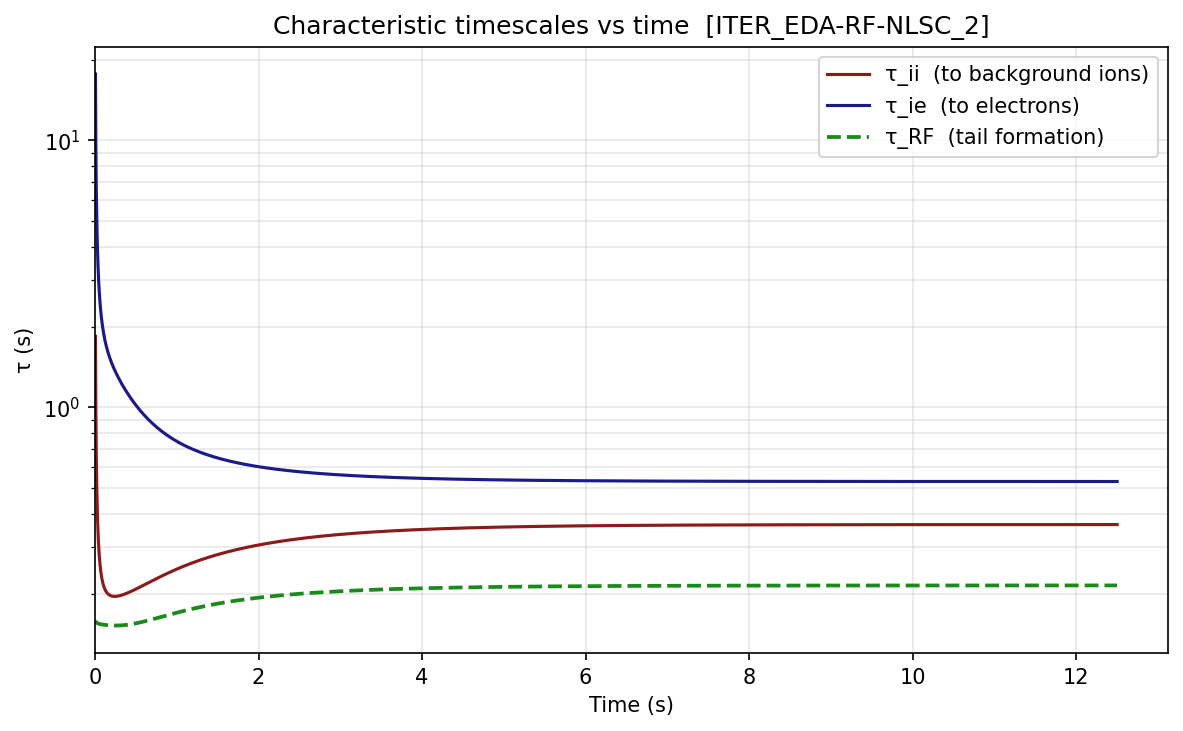
\includegraphics[width=\linewidth]{timescales_vs_time-ITER_EDA-RF-NLSC_2.png}
\caption{characteristic timescales}
\end{subfigure}
\caption{Power channels and the corresponding effective timescales
$\tau = n\Teff/P$. The identity $1/\tau_{\rm RF}=1/\tau_{ii}+1/\tau_{ie}$ holds
to $0.003\%$, which is the power balance restated.}
\label{fig:power}
\end{figure}

Read as timescales (Fig.~\ref{fig:power}, right), the RF fills the tail on
$\tau_{\rm RF}=0.216\,$s while the ions drain it on $\tau_{ii}=0.364\,$s and the
electrons on $\tau_{ie}=0.528\,$s. The RF is therefore the fastest process, by
a factor $1.7$ over the quicker of the two loss channels, which is why a
substantial supra-thermal population is sustained. All three fall steeply during
tail formation, since a cold minority stores little energy relative to the power
it can shed.

\vspace{-0.2cm}
\section{Summary and numerical quality}

\begin{table}[h]
\centering\small
\caption{Steady-state results.}
\begin{tabular}{@{}lr@{\hskip 2.2em}lr@{}}
\toprule
$\Teff$              & $32.59\,$keV            & $P_{\rm RF}$          & $1.8166\,$MW/m$^3$ \\
$T_n$                & $13.73\,$keV            & $P_{\rm coll}$ (ions) & $-1.0751\,$MW/m$^3$ \\
anisotropy           & $73.86\%$               & $P_{\rm coll}$ (elec.)& $-0.7415\,$MW/m$^3$ \\
$\tau_{\rm RF}$      & $0.2156\,$s             & $\tau_{ii}$           & $0.3643\,$s \\
$\tau_{ie}$          & $0.5281\,$s             & $E_c$                 & $106\,$keV \\
\bottomrule
\end{tabular}
\end{table}

The run stopped on the convergence criteria rather than exhausting its step
budget, and the residual drift in $\Teff$ over the final quarter of the run is
below $0.3\%$. The minority density changes by $+0.127\%$ over the whole run:
small, but not zero, and attributable to the slow particle gain of the
non-linear self-collision operator, whose rate scales with the minority density.
With the observed $\mathrm{d}\ln\Teff/\mathrm{d}\ln n\simeq-0.7$ this biases
$\Teff$ by under $0.1\%$. Wall truncation of $f$ is $4.9\times10^{-11}$ of the
peak, so the velocity domain is ample.

\vspace{0.2cm}
\noindent\footnotesize
Case \code{nominal\_\#2--REF}; figures from \code{figs/}, generated by
\code{fp2d\_plot.py} from the traces in \code{results/}.

\end{document}
